
%% bare_jrnl.tex
%% V1.3
%% 2007/01/11
%% by Michael Shell
%% see http://www.michaelshell.org/
%% for current contact information.
%%
%% This is a skeleton file demonstrating the use of IEEEtran.cls
%% (requires IEEEtran.cls version 1.7 or later) with an IEEE journal paper.
%%
%% Support sites:
%% http://www.michaelshell.org/tex/ieeetran/
%% http://www.ctan.org/tex-archive/macros/latex/contrib/IEEEtran/
%% and
%% http://www.ieee.org/



% *** Authors should verify (and, if needed, correct) their LaTeX system  ***
% *** with the testflow diagnostic prior to trusting their LaTeX platform ***
% *** with production work. IEEE's font choices can trigger bugs that do  ***
% *** not appear when using other class files.                            ***
% The testflow support page is at:
% http://www.michaelshell.org/tex/testflow/


%%*************************************************************************
%% Legal Notice:
%% This code is offered as-is without any warranty either expressed or
%% implied; without even the implied warranty of MERCHANTABILITY or
%% FITNESS FOR A PARTICULAR PURPOSE! 
%% User assumes all risk.
%% In no event shall IEEE or any contributor to this code be liable for
%% any damages or losses, including, but not limited to, incidental,
%% consequential, or any other damages, resulting from the use or misuse
%% of any information contained here.
%%
%% All comments are the opinions of their respective authors and are not
%% necessarily endorsed by the IEEE.
%%
%% This work is distributed under the LaTeX Project Public License (LPPL)
%% ( http://www.latex-project.org/ ) version 1.3, and may be freely used,
%% distributed and modified. A copy of the LPPL, version 1.3, is included
%% in the base LaTeX documentation of all distributions of LaTeX released
%% 2003/12/01 or later.
%% Retain all contribution notices and credits.
%% ** Modified files should be clearly indicated as such, including  **
%% ** renaming them and changing author support contact information. **
%%
%% File list of work: IEEEtran.cls, IEEEtran_HOWTO.pdf, bare_adv.tex,
%%                    bare_conf.tex, bare_jrnl.tex, bare_jrnl_compsoc.tex
%%*************************************************************************

% Note that the a4paper option is mainly intended so that authors in
% countries using A4 can easily print to A4 and see how their papers will
% look in print - the typesetting of the document will not typically be
% affected with changes in paper size (but the bottom and side margins will).
% Use the testflow package mentioned above to verify correct handling of
% both paper sizes by the user's LaTeX system.
%
% Also note that the "draftcls" or "draftclsnofoot", not "draft", option
% should be used if it is desired that the figures are to be displayed in
% draft mode.
%
\documentclass[journal]{IEEEtran}

% added by Zongxiao He, Oct 2nd, to save space
%\usepackage[
%top    = 2.00cm,
%bottom = 1.50cm,
%left   = 1.50cm,
%right  = 1.50cm]{geometry}

%
% If IEEEtran.cls has not been installed into the LaTeX system files,
% manually specify the path to it like:
% \documentclass[journal]{../sty/IEEEtran}





% Some very useful LaTeX packages include:
% (uncomment the ones you want to load)


% *** MISC UTILITY PACKAGES ***
%
%\usepackage{ifpdf}
% Heiko Oberdiek's ifpdf.sty is very useful if you need conditional
% compilation based on whether the output is pdf or dvi.
% usage:
% \ifpdf
%   % pdf code
% \else
%   % dvi code
% \fi
% The latest version of ifpdf.sty can be obtained from:
% http://www.ctan.org/tex-archive/macros/latex/contrib/oberdiek/
% Also, note that IEEEtran.cls V1.7 and later provides a builtin
% \ifCLASSINFOpdf conditional that works the same way.
% When switching from latex to pdflatex and vice-versa, the compiler may
% have to be run twice to clear warning/error messages.






% *** CITATION PACKAGES ***
%
%\usepackage{cite}
% cite.sty was written by Donald Arseneau
% V1.6 and later of IEEEtran pre-defines the format of the cite.sty package
% \cite{} output to follow that of IEEE. Loading the cite package will
% result in citation numbers being automatically sorted and properly
% "compressed/ranged". e.g., [1], [9], [2], [7], [5], [6] without using
% cite.sty will become [1], [2], [5]--[7], [9] using cite.sty. cite.sty's
% \cite will automatically add leading space, if needed. Use cite.sty's
% noadjust option (cite.sty V3.8 and later) if you want to turn this off.
% cite.sty is already installed on most LaTeX systems. Be sure and use
% version 4.0 (2003-05-27) and later if using hyperref.sty. cite.sty does
% not currently provide for hyperlinked citations.
% The latest version can be obtained at:
% http://www.ctan.org/tex-archive/macros/latex/contrib/cite/
% The documentation is contained in the cite.sty file itself.






% *** GRAPHICS RELATED PACKAGES ***
%
\ifCLASSINFOpdf
  \usepackage[pdftex]{graphicx}
  % declare the path(s) where your graphic files are
  % \graphicspath{{../pdf/}{../jpeg/}}
  % and their extensions so you won't have to specify these with
  % every instance of \includegraphics
  % \DeclareGraphicsExtensions{.pdf,.jpeg,.png}
\else
  % or other class option (dvipsone, dvipdf, if not using dvips). graphicx
  % will default to the driver specified in the system graphics.cfg if no
  % driver is specified.
  % \usepackage[dvips]{graphicx}
  % declare the path(s) where your graphic files are
  % \graphicspath{{../eps/}}
  % and their extensions so you won't have to specify these with
  % every instance of \includegraphics
  % \DeclareGraphicsExtensions{.eps}
\fi
% graphicx was written by David Carlisle and Sebastian Rahtz. It is
% required if you want graphics, photos, etc. graphicx.sty is already
% installed on most LaTeX systems. The latest version and documentation can
% be obtained at: 
% http://www.ctan.org/tex-archive/macros/latex/required/graphics/
% Another good source of documentation is "Using Imported Graphics in
% LaTeX2e" by Keith Reckdahl which can be found as epslatex.ps or
% epslatex.pdf at: http://www.ctan.org/tex-archive/info/
%
% latex, and pdflatex in dvi mode, support graphics in encapsulated
% postscript (.eps) format. pdflatex in pdf mode supports graphics
% in .pdf, .jpeg, .png and .mps (metapost) formats. Users should ensure
% that all non-photo figures use a vector format (.eps, .pdf, .mps) and
% not a bitmapped formats (.jpeg, .png). IEEE frowns on bitmapped formats
% which can result in "jaggedy"/blurry rendering of lines and letters as
% well as large increases in file sizes.
%
% You can find documentation about the pdfTeX application at:
% http://www.tug.org/applications/pdftex





% *** MATH PACKAGES ***
%
\usepackage[cmex10]{amsmath}
\usepackage{amssymb}

% A popular package from the American Mathematical Society that provides
% many useful and powerful commands for dealing with mathematics. If using
% it, be sure to load this package with the cmex10 option to ensure that
% only type 1 fonts will utilized at all point sizes. Without this option,
% it is possible that some math symbols, particularly those within
% footnotes, will be rendered in bitmap form which will result in a
% document that can not be IEEE Xplore compliant!
%
% Also, note that the amsmath package sets \interdisplaylinepenalty to 10000
% thus preventing page breaks from occurring within multiline equations. Use:
%\interdisplaylinepenalty=2500
% after loading amsmath to restore such page breaks as IEEEtran.cls normally
% does. amsmath.sty is already installed on most LaTeX systems. The latest
% version and documentation can be obtained at:
% http://www.ctan.org/tex-archive/macros/latex/required/amslatex/math/

% By Zongxiao He, for Fullpage table/picture in two column layout
% http://stackoverflow.com/questions/1856189/fullpage-picture-in-two-column-layout
% http://tex.stackexchange.com/questions/89462/page-wide-table-in-two-column-mode
\usepackage{multicol}



% *** SPECIALIZED LIST PACKAGES ***
%
%\usepackage{algorithmic}
% algorithmic.sty was written by Peter Williams and Rogerio Brito.
% This package provides an algorithmic environment fo describing algorithms.
% You can use the algorithmic environment in-text or within a figure
% environment to provide for a floating algorithm. Do NOT use the algorithm
% floating environment provided by algorithm.sty (by the same authors) or
% algorithm2e.sty (by Christophe Fiorio) as IEEE does not use dedicated
% algorithm float types and packages that provide these will not provide
% correct IEEE style captions. The latest version and documentation of
% algorithmic.sty can be obtained at:
% http://www.ctan.org/tex-archive/macros/latex/contrib/algorithms/
% There is also a support site at:
% http://algorithms.berlios.de/index.html
% Also of interest may be the (relatively newer and more customizable)
% algorithmicx.sty package by Szasz Janos:
% http://www.ctan.org/tex-archive/macros/latex/contrib/algorithmicx/




% *** ALIGNMENT PACKAGES ***
%
\usepackage{array}
\usepackage{tabularx}
\usepackage{booktabs}
\usepackage{multirow}
\usepackage{makecell}
\usepackage[ruled,vlined]{algorithm2e}
% Frank Mittelbach's and David Carlisle's array.sty patches and improves
% the standard LaTeX2e array and tabular environments to provide better
% appearance and additional user controls. As the default LaTeX2e table
% generation code is lacking to the point of almost being broken with
% respect to the quality of the end results, all users are strongly
% advised to use an enhanced (at the very least that provided by array.sty)
% set of table tools. array.sty is already installed on most systems. The
% latest version and documentation can be obtained at:
% http://www.ctan.org/tex-archive/macros/latex/required/tools/


%\usepackage{mdwmath}
%\usepackage{mdwtab}
% Also highly recommended is Mark Wooding's extremely powerful MDW tools,
% especially mdwmath.sty and mdwtab.sty which are used to format equations
% and tables, respectively. The MDWtools set is already installed on most
% LaTeX systems. The lastest version and documentation is available at:
% http://www.ctan.org/tex-archive/macros/latex/contrib/mdwtools/


% IEEEtran contains the IEEEeqnarray family of commands that can be used to
% generate multiline equations as well as matrices, tables, etc., of high
% quality.


%\usepackage{eqparbox}
% Also of notable interest is Scott Pakin's eqparbox package for creating
% (automatically sized) equal width boxes - aka "natural width parboxes".
% Available at:
% http://www.ctan.org/tex-archive/macros/latex/contrib/eqparbox/





% *** SUBFIGURE PACKAGES ***
%\usepackage[tight,footnotesize]{subfigure}
% subfigure.sty was written by Steven Douglas Cochran. This package makes it
% easy to put subfigures in your figures. e.g., "Figure 1a and 1b". For IEEE
% work, it is a good idea to load it with the tight package option to reduce
% the amount of white space around the subfigures. subfigure.sty is already
% installed on most LaTeX systems. The latest version and documentation can
% be obtained at:
% http://www.ctan.org/tex-archive/obsolete/macros/latex/contrib/subfigure/
% subfigure.sty has been superceeded by subfig.sty.



%\usepackage[caption=false]{caption}
%\usepackage[font=footnotesize]{subfig}
% subfig.sty, also written by Steven Douglas Cochran, is the modern
% replacement for subfigure.sty. However, subfig.sty requires and
% automatically loads Axel Sommerfeldt's caption.sty which will override
% IEEEtran.cls handling of captions and this will result in nonIEEE style
% figure/table captions. To prevent this problem, be sure and preload
% caption.sty with its "caption=false" package option. This is will preserve
% IEEEtran.cls handing of captions. Version 1.3 (2005/06/28) and later 
% (recommended due to many improvements over 1.2) of subfig.sty supports
% the caption=false option directly:
%\usepackage[caption=false,font=footnotesize]{subfig}
%
% The latest version and documentation can be obtained at:
% http://www.ctan.org/tex-archive/macros/latex/contrib/subfig/
% The latest version and documentation of caption.sty can be obtained at:
% http://www.ctan.org/tex-archive/macros/latex/contrib/caption/




% *** FLOAT PACKAGES ***
%
%\usepackage{fixltx2e}
% fixltx2e, the successor to the earlier fix2col.sty, was written by
% Frank Mittelbach and David Carlisle. This package corrects a few problems
% in the LaTeX2e kernel, the most notable of which is that in current
% LaTeX2e releases, the ordering of single and double column floats is not
% guaranteed to be preserved. Thus, an unpatched LaTeX2e can allow a
% single column figure to be placed prior to an earlier double column
% figure. The latest version and documentation can be found at:
% http://www.ctan.org/tex-archive/macros/latex/base/



%\usepackage{stfloats}
% stfloats.sty was written by Sigitas Tolusis. This package gives LaTeX2e
% the ability to do double column floats at the bottom of the page as well
% as the top. (e.g., "\begin{figure*}[!b]" is not normally possible in
% LaTeX2e). It also provides a command:
%\fnbelowfloat
% to enable the placement of footnotes below bottom floats (the standard
% LaTeX2e kernel puts them above bottom floats). This is an invasive package
% which rewrites many portions of the LaTeX2e float routines. It may not work
% with other packages that modify the LaTeX2e float routines. The latest
% version and documentation can be obtained at:
% http://www.ctan.org/tex-archive/macros/latex/contrib/sttools/
% Documentation is contained in the stfloats.sty comments as well as in the
% presfull.pdf file. Do not use the stfloats baselinefloat ability as IEEE
% does not allow \baselineskip to stretch. Authors submitting work to the
% IEEE should note that IEEE rarely uses double column equations and
% that authors should try to avoid such use. Do not be tempted to use the
% cuted.sty or midfloat.sty packages (also by Sigitas Tolusis) as IEEE does
% not format its papers in such ways.


%\ifCLASSOPTIONcaptionsoff
%  \usepackage[nomarkers]{endfloat}
% \let\MYoriglatexcaption\caption
% \renewcommand{\caption}[2][\relax]{\MYoriglatexcaption[#2]{#2}}
%\fi
% endfloat.sty was written by James Darrell McCauley and Jeff Goldberg.
% This package may be useful when used in conjunction with IEEEtran.cls'
% captionsoff option. Some IEEE journals/societies require that submissions
% have lists of figures/tables at the end of the paper and that
% figures/tables without any captions are placed on a page by themselves at
% the end of the document. If needed, the draftcls IEEEtran class option or
% \CLASSINPUTbaselinestretch interface can be used to increase the line
% spacing as well. Be sure and use the nomarkers option of endfloat to
% prevent endfloat from "marking" where the figures would have been placed
% in the text. The two hack lines of code above are a slight modification of
% that suggested by in the endfloat docs (section 8.3.1) to ensure that
% the full captions always appear in the list of figures/tables - even if
% the user used the short optional argument of \caption[]{}.
% IEEE papers do not typically make use of \caption[]'s optional argument,
% so this should not be an issue. A similar trick can be used to disable
% captions of packages such as subfig.sty that lack options to turn off
% the subcaptions:
% For subfig.sty:
% \let\MYorigsubfloat\subfloat
% \renewcommand{\subfloat}[2][\relax]{\MYorigsubfloat[]{#2}}
% For subfigure.sty:
% \let\MYorigsubfigure\subfigure
% \renewcommand{\subfigure}[2][\relax]{\MYorigsubfigure[]{#2}}
% However, the above trick will not work if both optional arguments of
% the \subfloat/subfig command are used. Furthermore, there needs to be a
% description of each subfigure *somewhere* and endfloat does not add
% subfigure captions to its list of figures. Thus, the best approach is to
% avoid the use of subfigure captions (many IEEE journals avoid them anyway)
% and instead reference/explain all the subfigures within the main caption.
% The latest version of endfloat.sty and its documentation can obtained at:
% http://www.ctan.org/tex-archive/macros/latex/contrib/endfloat/
%
% The IEEEtran \ifCLASSOPTIONcaptionsoff conditional can also be used
% later in the document, say, to conditionally put the References on a 
% page by themselves.





% *** PDF, URL AND HYPERLINK PACKAGES ***
%
%\usepackage{url}
% url.sty was written by Donald Arseneau. It provides better support for
% handling and breaking URLs. url.sty is already installed on most LaTeX
% systems. The latest version can be obtained at:
% http://www.ctan.org/tex-archive/macros/latex/contrib/misc/
% Read the url.sty source comments for usage information. Basically,
% \url{my_url_here}.





% *** Do not adjust lengths that control margins, column widths, etc. ***
% *** Do not use packages that alter fonts (such as pslatex).         ***
% There should be no need to do such things with IEEEtran.cls V1.6 and later.
% (Unless specifically asked to do so by the journal or conference you plan
% to submit to, of course. )


% correct bad hyphenation here
\hyphenation{op-tical net-works semi-conduc-tor}


\begin{document}
%
% paper title
% can use linebreaks \\ within to get better formatting as desired
\title{A Combined Collaborative Filtering Model for Recommender System}
%
%
% author names and IEEE memberships
% note positions of commas and nonbreaking spaces ( ~ ) LaTeX will not break
% a structure at a ~ so this keeps an author's name from being broken across
% two lines.
% use \thanks{} to gain access to the first footnote area
% a separate \thanks must be used for each paragraph as LaTeX2e's \thanks
% was not built to handle multiple paragraphs
%

\author{Team {\it 1UP+}: Di Fu$^{\dagger}$~and~Zongxiao He$^{\ddagger}$% <-this % stops a space
\thanks{$^{\dagger}$Department of Statistics, Rice University, df14@rice.edu.}
\thanks{$^{\ddagger}$Department of Genetics, Baylor College of Medicine, zh6@rice.edu.}}

% note the % following the last \IEEEmembership and also \thanks - 
% these prevent an unwanted space from occurring between the last author name
% and the end of the author line. i.e., if you had this:
% 
% \author{....lastname \thanks{...} \thanks{...} }
%                     ^------------^------------^----Do not want these spaces!
%
% a space would be appended to the last name and could cause every name on that
% line to be shifted left slightly. This is one of those "LaTeX things". For
% instance, "\textbf{A} \textbf{B}" will typeset as "A B" not "AB". To get
% "AB" then you have to do: "\textbf{A}\textbf{B}"
% \thanks is no different in this regard, so shield the last } of each \thanks
% that ends a line with a % and do not let a space in before the next \thanks.
% Spaces after \IEEEmembership other than the last one are OK (and needed) as
% you are supposed to have spaces between the names. For what it is worth,
% this is a minor point as most people would not even notice if the said evil
% space somehow managed to creep in.



% The paper headers
\markboth{Rice STAT640: Data Mining and Statistical Learning,~Team {\it ~1UP+}  Report, 2013}%
{Shell \MakeLowercase{\textit{et al.}}: Bare Demo of IEEEtran.cls for Journals}
% The only time the second header will appear is for the odd numbered pages
% after the title page when using the twoside option.
% 
% *** Note that you probably will NOT want to include the author's ***
% *** name in the headers of peer review papers.                   ***
% You can use \ifCLASSOPTIONpeerreview for conditional compilation here if
% you desire.




% If you want to put a publisher's ID mark on the page you can do it like
% this:
%\IEEEpubid{0000--0000/00\$00.00~\copyright~2007 IEEE}
% Remember, if you use this you must call \IEEEpubidadjcol in the second
% column for its text to clear the IEEEpubid mark.



% use for special paper notices
%\IEEEspecialpapernotice{(Invited Paper)}


% make the title area
\maketitle

\begin{abstract}
%\boldmath
Collaborative filtering is a widely used and sucessful recommendation paradigm that models users\rq{} collaborative behaviors reflected in previous transactions for recommendation. Neighborhood model and latent factor model are most common approaches to collaborative filtering. In this project, we build several rating prediction models based upon neighborhood model and latent factor model and applied them on the MovieLens dataset. We evaluated the performance each model and ensembled a final model to predict a numerical rating for each missed entry in MovieLens dataset.
 
\end{abstract}
% IEEEtran.cls defaults to using nonbold math in the Abstract.
% This preserves the distinction between vectors and scalars. However,
% if the journal you are submitting to favors bold math in the abstract,
% then you can use LaTeX's standard command \boldmath at the very start
% of the abstract to achieve this. Many IEEE journals frown on math
% in the abstract anyway.

% Note that keywords are not normally used for peerreview papers.
%\begin{IEEEkeywords}
%IEEEtran, journal, \LaTeX, paper, template.
%\end{IEEEkeywords}





% For peer review papers, you can put extra information on the cover
% page as needed:
% \ifCLASSOPTIONpeerreview
% \begin{center} \bfseries EDICS Category: 3-BBND \end{center}
% \fi
%
% For peerreview papers, this IEEEtran command inserts a page break and
% creates the second title. It will be ignored for other modes.
\IEEEpeerreviewmaketitle



%\section{Introduction}
% The very first letter is a 2 line initial drop letter followed
% by the rest of the first word in caps.
% 
% form to use if the first word consists of a single letter:
% \IEEEPARstart{A}{demo} file is ....
% 
% form to use if you need the single drop letter followed by
% normal text (unknown if ever used by IEEE):
% \IEEEPARstart{A}{}demo file is ....
% 
% Some journals put the first two words in caps:
% \IEEEPARstart{T}{his demo} file is ....
% 
% Here we have the typical use of a "T" for an initial drop letter
% and "HIS" in caps to complete the first word.
%\IEEEPARstart{R}{}ecommender systems use the personal information of a user (i.e., the user\rq{}s rates on all movies he/she has seen) to uncover his perference or hibits and consider this information in the product suggestion. Collaborative filtering is a widely used and sucessful recommendation paradigm that models users\rq{} collaborative behaviors reflected in transactions.  In this project, we will build a rating prediction model which is based on collaborative filtering model for a dataset of users and movies from movielens.org. 

%\hfill mds
%\hfill January 11, 2007

%\subsection{Previous Work}
%Subsection text here.
%
%% needed in second column of first page if using \IEEEpubid
%%\IEEEpubidadjcol
%
%\subsection{Our Project}
%Subsection text here.


\section{Dataset}
The MovieLens academic dataset provides ratings of the 6,040 users to 3,187 movies (Figure~\ref{fig1}). The Whole Training Set (WTS) available to students includes 801,051 ($4.15\%$) ratings, user meta-data (gender, age, and occupation), and movie meta-data (name and genres). Ratings are integers between 1 to 5. The Qualifying Set on Kaggle is split into two parts: Quiz set, which is used for evaluate the submission in public leaderboard, and Test Set, which will be used for calculating final score. For the purpose of training and comparing models, the hand-out WTS is split randomly into Training Set (TS, $\sim97\%$ of WTS) and Probe Set ($\sim3\%$ of WTS). 
\begin{figure}[ht]
\begin{center}
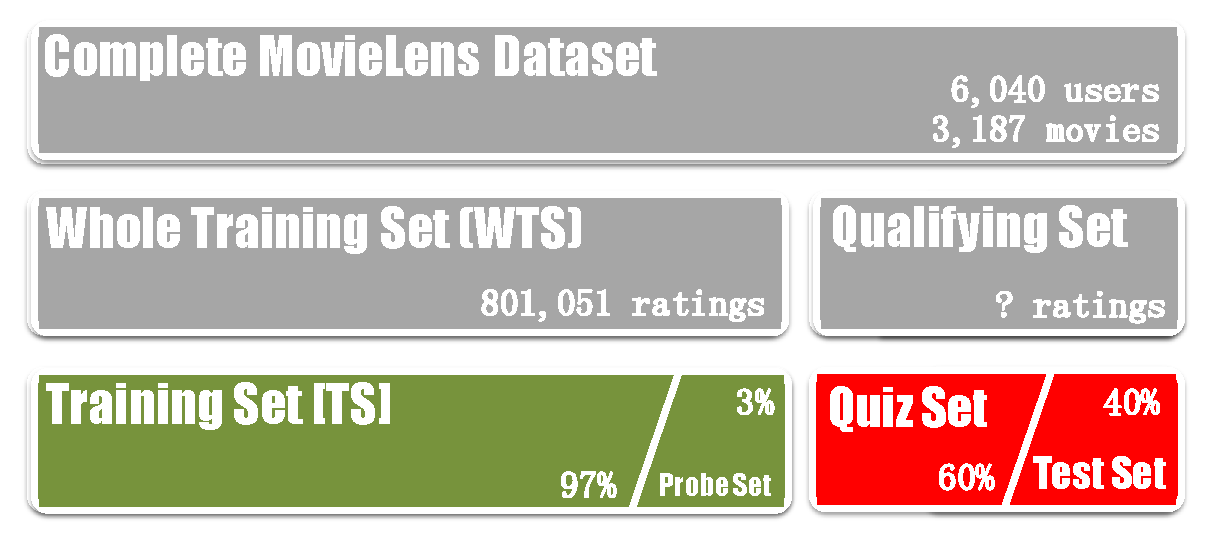
\includegraphics[width=3.2in]{fig/dataset}
\caption{The structure of MovieLens dataset. }
\label{fig1}
\end{center}
\end{figure}

We model users and movies as nodes, with ratings as directed edges. The distributions of some statistics about this dataset are shown in Figure~\ref{fig2}. The ratings tend to more positive than negative (right panel). A important fact about this dataset is that the variance of average rating per movie (left panel) is significantly larger than that of average rating per movie (middle panel), which suggests more information is hidden under item-item pairs.

\begin{figure}[ht]
\begin{center}$
\begin{array}{cc}
%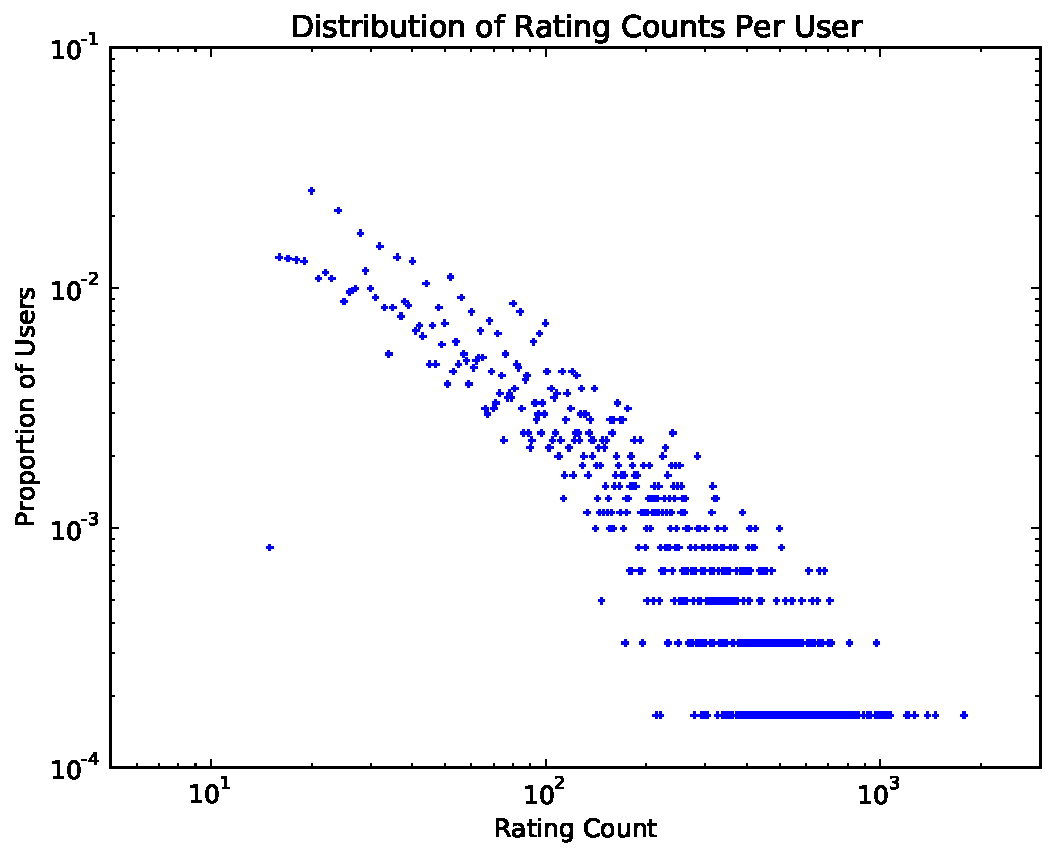
\includegraphics[width=1.1in]{user_rating_count}
%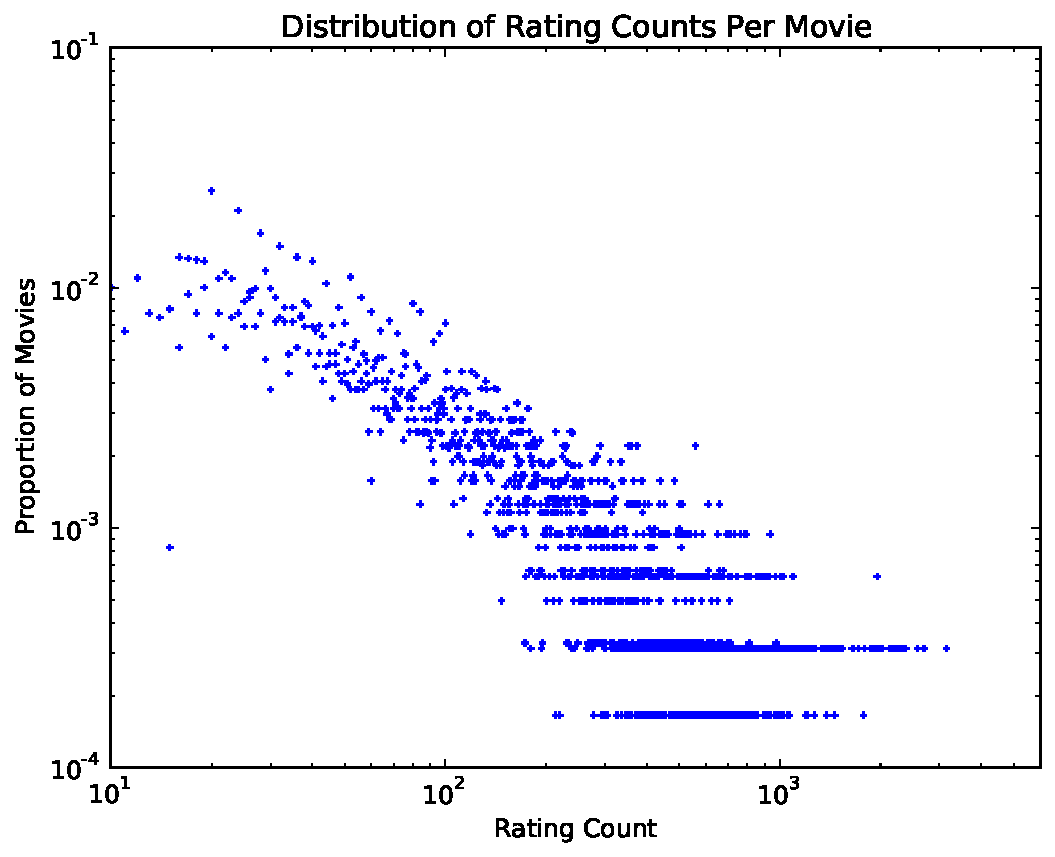
\includegraphics[width=1.1in]{item_rating_count} \\
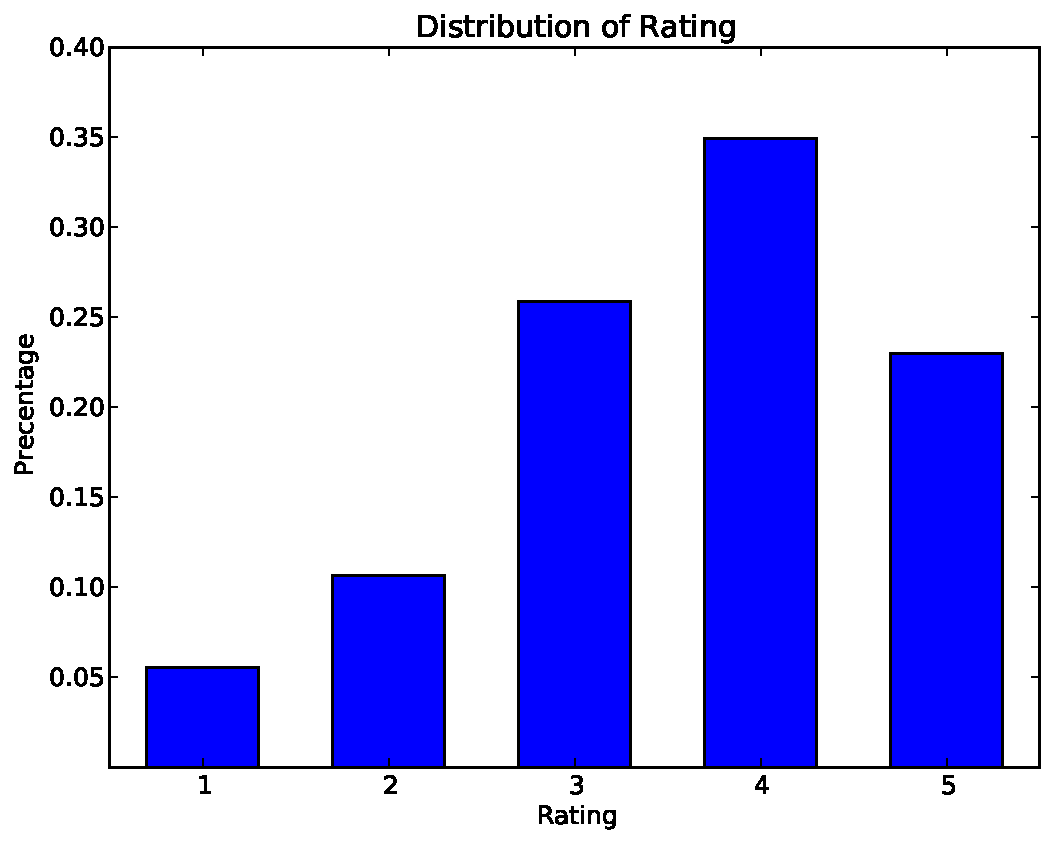
\includegraphics[width=1.1in]{fig/rating_hist}
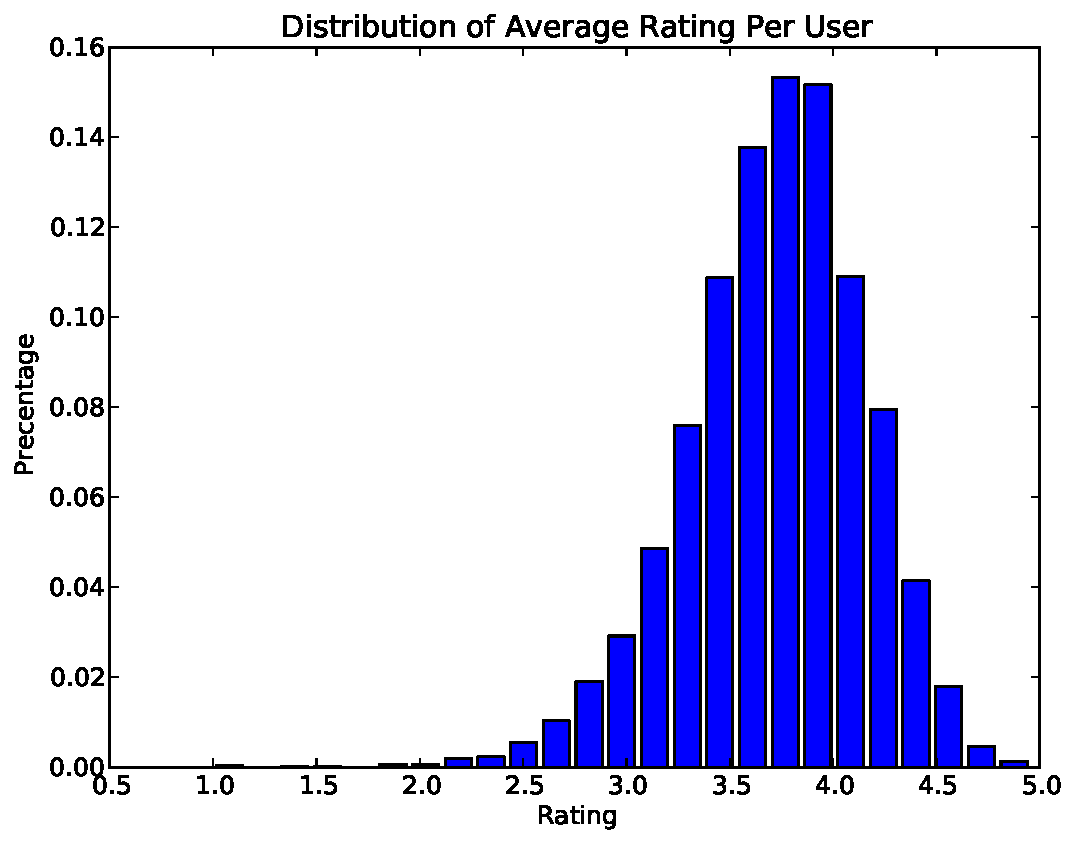
\includegraphics[width=1.1in]{fig/user_aver_rating}
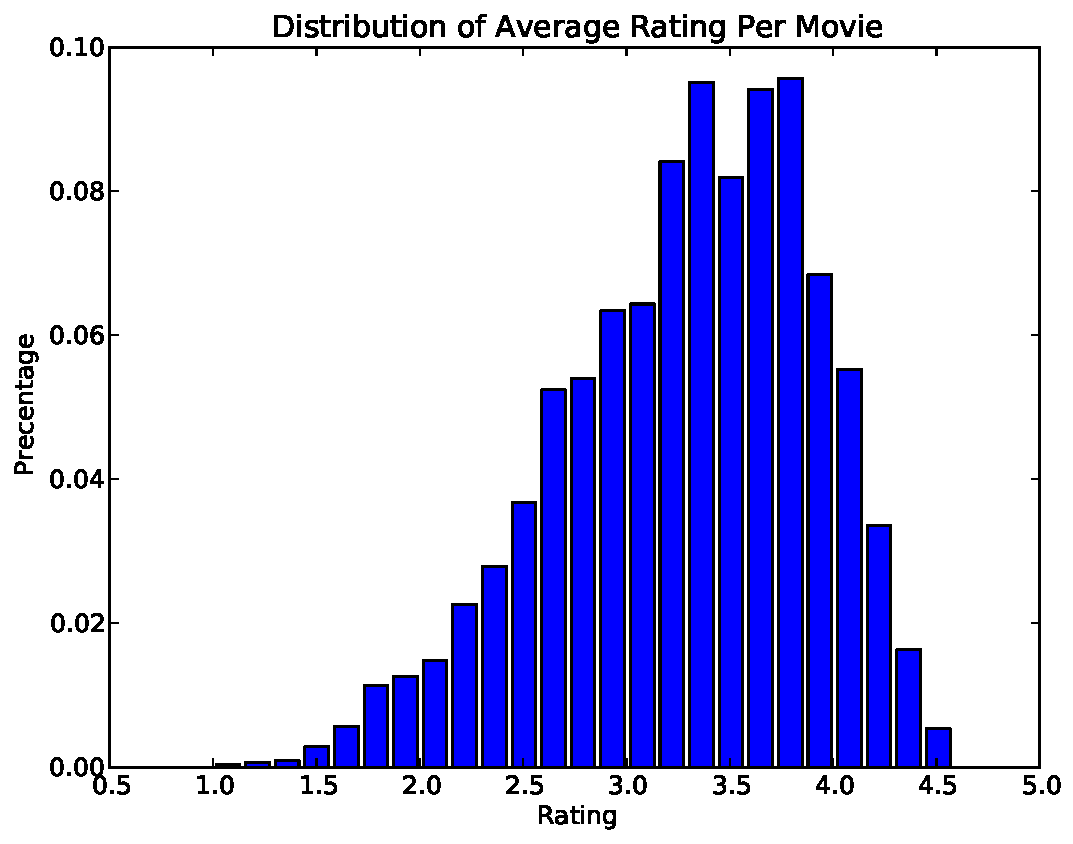
\includegraphics[width=1.1in]{fig/movie_aver_rating}
\end{array}$
\vspace{-2mm}
\caption{{\it Left To Right}: Distribution of Rating, Distribution of User Average Rating, Distribution of Movie Average Rating. }
\label{fig2}
\end{center}
\end{figure}

%{\it Top Row, Left to Right}: Degree Distribution of User Rating Counts, Degree Distribution of Movie Rating Counts. 

\section{Methodology}

\subsection{Notations}

$u$ and $v$ will be reserved as indexing letters for users, as for items(movies) $i$ and $j$. $r_{ui}$ indicates the rating by user $u$ for item $i$, and $\hat{r}_{ui}$ is the predicated value of it. The set of $(u,i)$ pairs in which $r_{ui}$ is known is $K = \{(u,i) | r_{u,i} $ is know$\}$. Regularization parameters are denoted as $\lambda_1, \lambda_2, \ldots$ and step sizes are denoted as $\gamma_1, \gamma_2, \ldots$. The root mean square error on Probe Set is denoted as Probe\_RMSE and will be used to measure the convergence of our iterative optimization algorithms.  The average of root mean square error in cross validation is denoted as mean\_RMSE and will be used for model selection.

\subsection{Parameter selection}
Each models we developed has dataset dependent parameters (e.g. regularization, step size, number of features etc). In order to select the correct ones, we use an approach including three-round grid search and an 10-fold cross validation.  Starting with a wide range ($[0.0005, 0.05]$ for $\lambda$'s and $\gamma$'s, $[50,400]$ for number of features), each round of grid search narrows down the parameter spaces. The best 30 parameter sets (defined as smallest Probe\_RMSEs) of last round grid search will be evaluated using 10-fold cross validation, and the optimal parameter sets are chosen by smallest mean\_RMSEs.

\subsection{Baseline Model}
To adjust user-specific and item-specific effects, the baseline estimate $b_{ui}$ of rating $r_{ui}$ is given as
\begin{align}
\label{eq1}
{b}_{ui} = \bar{r} + b_u + b_i
\end{align}
where $\bar{r}$ is the global average rating, $b_u$ and $b_i$ are user bias and movie bias \cite{koren}.

The  $b_u$ and $b_i$ can be calculated by solving the least squares problem:
\begin{align}
\label{eq2}
\min_{b_*}  & \sum_{(u,i) \in K} ( r_{ui} - \bar{r} - b_u - b_i )^2  + \lambda_1 (\sum_u b_u^2 + \sum_i b_i^2)
\end{align}
 
Instead of directly solving the equation (\ref{eq2}), the $b_u$ and $b_i$ can be estimated via gradient descent method, as shown in algorithm~\ref{alg1}. 

\begin{algorithm}[ht]
 \SetAlgoLined  % doesn't work in home computer (version of algo package)
 \textbf{Input:} {Training data $K$; $\gamma_1$; $\lambda_1$.} \\
 \textbf{Output:} {$b_*$; $Probe\_RMSE$.} \\
 \While{Probe\_RMSE keep decreasing}{
 
	\For{ $(u,i) \in K$ }{
        $e_{ui} := r_{ui} - \hat{r}_{ui}$ \\
        $b_u \gets b_u + \gamma_1 \cdot (e_{ui} - \lambda_1 \cdot b_u)$ \\
        $b_i \gets b_i + \gamma_1 \cdot (e_{ui} - \lambda_1 \cdot b_i)$ \\
   }
   
 	${ \gamma_1} \gets { \gamma_1} \times 0.9$ \\
 	calculate $Probe\_RMSE$
 }

 \caption{Baseline model algorithm}
\label{alg1}
\end{algorithm}

\subsection{Global neighborhood (GN) model}
\subsubsection{Neighborhood model}
Neighborhood model is very effective at detecting very localized relationships and rely on a few significant neighborhood relations. The item-oriented neighborhood \cite{item} is given as
\begin{align}
\label{eq3}
\hat{r}_{ui} = \bar{r} + b_u + b_i + \frac{\sum_{j \in S^k(i;u)} (r_{uj} - b_{uj}) \cdot s_{ij}}{\sum_{j \in S^z(i;u)} s_{ij}}
\end{align}
where $S^z(i;u)$ denotes the "neighbors", which is defined as $z$ items rated by $u$ and most similar to $i$. The $s_{ij}$ is the Pearson correlation coefficient that measures the tendency of users to rate movie $i$ and movie $j$ similarly.

Model defined in (\ref{eq2}) is fully rely on the neighbors, since the interpolation weights sum to one. This would be problematic in cases where neighborhood information is absent. An improved model \cite{koren} is suggested as
\begin{align}
\label{eq4}
\hat{r}_{ui} = \bar{r} + b_u + b_i + \sum_{j \in R(u)} (r_{uj} - b_{uj}) \cdot w_{ij}
\end{align}
where $R(u)$ is the set of items rated by user $u$. The user-specific interpolation weight ${s_{ij}}/{\sum_{j \in S^z(i;u)} s_{ij}}$ is replaced by $w_{ij}$, which denote the global weight from $j$ to $i$ and is learned from the data through optimization. 

\subsubsection{Implicit feedback} 
An important lesson from the Netflix Prize competition is the importance of integrating different forms of implicit feedbacks, such as purchase history, browsing history, search patterns\cite{lesson}. The MovieLens dataset does not only tell us the rating values, but also which movies users rate, regardless of how they rated these movies. It has been shown that incorporating this kind of implicit data significantly improved prediction accuracy \cite{koren}.

Following up model (\ref{eq4}), implicit feedback can be added as another set of weights,
\begin{align}
\label{eq5}
\hat{r}_{ui} = & \bar{r} + b_u + b_i + \sum_{j \in R(u)} (r_{uj} - b_{uj}) \cdot w_{ij}  + \sum_{j \in N(u)}  c_{ij}
\end{align}
where $N(u)$ contains all items for which $u$ provided an implicit preference. $c_{ij}$ is offset added to baseline estimates, which is expected to be high if $j$ is predictive on $i$.  

To avoid the great deviations from baseline estimates for users that provided many ratings or plenty of implicit feedback, add an regularization item to the model (\ref{eq5}) as
\begin{align}
\label{eq6}
\hat{r}_{ui} = & \bar{r} + b_u + b_i + |R(u)|^{-\frac{1}{2}} \sum_{j \in R(u)} (r_{uj} - b_{uj}) \cdot w_{ij}  \notag \\
& + |N(u)|^{-\frac{1}{2}} \sum_{j \in N(u)}  c_{ij}
\end{align}

The  model (\ref{eq6}) can be learned by solving the regularized least squares problem
\begin{align}
\label{eq7}
\min_{b_*, w_*, c_*}  & \sum_{(u,i) \in K} \Big( r_{ui} - \bar{r} - b_u - b_i - |R(u)|^{-\frac{1}{2}} \sum_{j \in R(u)} \notag \\
& (r_{uj} - b_{uj}) \cdot w_{ij} -  |N(u)|^{-\frac{1}{2}} \sum_{j \in N(u)}  c_{ij} \Big)^2 \notag \\
& + \lambda_3 (b_u^2 + b_i^2 +\sum w_{ij}^2 + \sum c_{ij}^2)
\end{align}

A gradient descent solver for this optimization problem (\ref{eq7}) is shown in algorithm~\ref{alg2}.

\begin{algorithm}[ht]
 \SetAlgoLined  % doesn't work in home computer (version of algo package)
 \textbf{Input:} {Training data $K$;$\gamma_1, \gamma_3$; $\lambda_1, \lambda_3$.} \\
 \textbf{Output:} {$b_*, w_*, c_*$; $Probe\_RMSE$.} \\
 \While{Probe\_RMSE keep decreasing}{
 
	\For{ $(u,i) \in K$ }{
        $e_{ui} := r_{ui} - \hat{r}_{ui}$ \\
        $b_u \gets b_u + \gamma_1 \cdot (e_{ui} - \lambda_1 \cdot b_u)$ \\
        $b_i \gets b_i + \gamma_1 \cdot (e_{ui} - \lambda_1 \cdot b_i)$ \\
   		\For{ $j \in R(u)$ }{
        $w_{ij} \gets w_{ij} + \gamma_3 \cdot (e_{ui} \cdot |R(u)|^{-\frac{1}{2}} \cdot (r_{uj} - b_{uj}) - \lambda_3 \cdot w_{ij})$ 
   		}
   		\For{ $j \in N(u)$ }{
        $c_{ij} \gets c_{ij} + \gamma_3 \cdot (e_{ui} \cdot |N(u)|^{-\frac{1}{2}} - \lambda_3 \cdot c_{ij})$ 
   		}
   }
   
 	${\boldsymbol \gamma} \gets {\boldsymbol \gamma} \times 0.9$ \\
 	calculate $Probe\_RMSE$
 }

 \caption{GN model algorithm}
\label{alg2}
\end{algorithm}

\subsection{Singular value decomposition (SVD) model}
Latent factor model is another most common approach to collaborative filtering. An drawback of neighborhood model is that it ignores the vast majority of ratings by a user and therefore it's unable to capture the totality of weak signals encompassed in all of a user\rq{}s ratings. Latent factor models are generally effective at estimating overall structure that relates simultaneously to most or all items.  We will focus on models that are induced by Singular Value Decomposition (SVD) on the user-item ratings matrix.

In this model, each user $u$ is associated with a user-factors vector $p_u \in \mathbb R^k$, and each item $i$ with an item-factors vector $q_i \in \mathbb R^k$. The prediction rule is
\begin{align}
\label{eq8}
\hat{r}_{ui} = & \bar{r} + b_u + b_i + p_u^T q_i
\end{align}

Simon Funk\cite{svd} introduced a gradient descent optimization approach (shown in algorithm~\ref{alg3}) to learn parameters that minimized the associated squared error 
\begin{align}
\label{eq9}
\min_{b_*, q_*, p_*}  & \sum_{(u,i) \in K} \Big( r_{ui} - \bar{r} - b_u - b_i - p_u^T q_i \Big)^2 \notag \\
& + \lambda_2 (b_u^2 + b_i^2 + ||p_u||^2 +  ||q_i||^2)
\end{align}

\begin{algorithm}[ht]
 \SetAlgoLined  % doesn't work in home computer (version of algo package)
 \textbf{Input:} {Training data $K$; k; $\gamma_1, \gamma_2$; $\lambda_1, \lambda_2$.} \\
 \textbf{Output:} {$b_*, q_*, p_*$; $Probe\_RMSE$.} \\
 \While{Probe\_RMSE keep decreasing}{
 
	\For{ $(u,i) \in K$ }{
        $e_{ui} := r_{ui} - \hat{r}_{ui}$ \\
        $b_u \gets b_u + \gamma_1 \cdot (e_{ui} - \lambda_1 \cdot b_u)$ \\
        $b_i \gets b_i + \gamma_1 \cdot (e_{ui} - \lambda_1 \cdot b_i)$ \\
        $q_i \gets q_i + \gamma_2 \cdot (e_{ui} \cdot p_u  - \lambda_2 \cdot q_i)$ \\
        $p_u \gets p_u + \gamma_2 \cdot (e_{ui} \cdot q_i - \lambda_2 \cdot p_u)$ \\
   }
   
 	${\boldsymbol \gamma} \gets {\boldsymbol \gamma} \times 0.9$ \\
 	calculate $Probe\_RMSE$
 }

 \caption{SVD model algorithm}
\label{alg3}
\end{algorithm}

\subsection{Asymmetric-SVD (SVDasym) model}

In the plain SVD model, a user is represented by the feature vector $q_u$. An extended SVD model integrating neighborhood relationship and implicit feedback is suggested by Paterek \cite{Paterek} and Koren \cite{koren} is given as
\begin{align}
\label{eq10}
\hat{r}_{ui} = & \bar{r} + b_u + b_i + |R(u)|^{-\frac{1}{2}} \sum_{j \in R(u)} (r_{uj} - b_{uj})  q_i^T x_{i} \notag \\
& +  |N(u)|^{-\frac{1}{2}} \sum_{j \in N(u)}  q_i^T y_{j} \notag \\
= & \bar{r} + b_u + b_i +  q_i^T\Big(|R(u)|^{-\frac{1}{2}} \sum_{j \in R(u)} (r_{uj} - b_{uj})  x_{j} \notag \\
& +  |N(u)|^{-\frac{1}{2}} \sum_{j \in N(u)}  y_{j} \Big)
\end{align}
where $y_j \in \mathbb R^k$ is factor vector associated with item $j$ representing implicit feedback.  A gradient descent appraoch given in algorithm~\ref{alg4} can be employed to solve the system.
\begin{algorithm}[ht]
 \SetAlgoLined  % doesn't work in home computer (version of algo package)
 \textbf{Input:} {Training data $K$; k; $\gamma_1, \gamma_2$; $\lambda_1, \lambda_2$.} \\
 \textbf{Output:} {$b_*, q_*, x_*, y_*$; $Probe\_RMSE$.} \\
 \While{Probe\_RMSE keep decreasing}{
 
	\For{ $u = 1,\ldots, m$ }{
        $p_u \gets |R(u)|^{-\frac{1}{2}} \sum_{j \in R(u)} (r_{uj} - b_{uj}) * x_{j}  +  |N(u)|^{-\frac{1}{2}} \sum_{j \in N(u)}  y_{j} $ \\
	 $sum \gets 0 $ \\
	
	\For{ $i \in R(u)$ }{
        $e_{ui} := r_{ui} - \hat{r}_{ui}$ \\
        $b_u \gets b_u + \gamma_1 \cdot (e_{ui} - \lambda_1 \cdot b_u)$ \\
        $b_i \gets b_i + \gamma_1 \cdot (e_{ui} - \lambda_1 \cdot b_i)$ \\
        $q_i \gets q_i + \gamma_2 \cdot (e_{ui} \cdot  p_u  - \lambda_2 \cdot q_i)$ \\
        }
     
	\For{ $j \in R(u)$ }{
        $x_j \gets x_j + \gamma_2 \cdot \big( |N(u)|^{-\frac{1}{2}} \cdot (r_{uj} - b_{uj}) \cdot sum - \lambda_2 \cdot x_j \big)$ 
        }
   
        \For{ $j \in N(u)$ }{
        $y_j \gets y_j + \gamma_2 \cdot (|N(u)|^{-\frac{1}{2}} \cdot sum - \lambda_2 \cdot y_i)$ 
   		}
   }
   
 	${\boldsymbol \gamma} \gets {\boldsymbol \gamma} \times 0.9$ \\
 	calculate $Probe\_RMSE$
 }


 \caption{SVDasym model algorithm}
\label{alg4}
\end{algorithm}


\subsection{SVD++ model}
Koren \cite{koren} proposed a more direct modification of model (\ref{eq8}) to integration of implicit feedback, and the model is given as
\begin{align}
\label{eq11}
\hat{r}_{ui} = & \bar{r} + b_u + b_i +  q_i^T\Big(p_u +  |N(u)|^{-\frac{1}{2}} \sum_{j \in N(u)}  y_{j} \Big)
\end{align}

Model can be trained by minimizing the associated squared error function through gradient descent, as shown in algorithm~\ref{alg5}.

\begin{algorithm}[ht]
 \SetAlgoLined  % doesn't work in home computer (version of algo package)
 \textbf{Input:} {Training data $K$; k; $\gamma_1, \gamma_2$; $\lambda_1, \lambda_2$.} \\
 \textbf{Output:} {$b_*, q_*, p_*, y_*$; $Probe\_RMSE$.} \\
 \While{Probe\_RMSE keep decreasing}{
 
	\For{ $(u,i) \in K$ }{
        $e_{ui} := r_{ui} - \hat{r}_{ui}$ \\
        $b_u \gets b_u + \gamma_1 \cdot (e_{ui} - \lambda_1 \cdot b_u)$ \\
        $b_i \gets b_i + \gamma_1 \cdot (e_{ui} - \lambda_1 \cdot b_i)$ \\
        $q_i \gets q_i + \gamma_2 \cdot (e_{ui} \cdot ( p_u + |N(u)|^{-\frac{1}{2}} \sum_{j \in N(u)}  y_{j}) - \lambda_2 \cdot q_i)$ \\
        $p_u \gets p_u + \gamma_2 \cdot (e_{ui} \cdot q_i - \lambda_2 \cdot p_u)$ \\
        
        \For{ $j \in N(u)$ }{
        $y_j \gets y_j + \gamma_2 \cdot (e_{ui} \cdot |N(u)|^{-\frac{1}{2}} \cdot q_i - \lambda_2 \cdot y_i)$ 
   		}
   }
   
 	${\boldsymbol \gamma} \gets {\boldsymbol \gamma} \times 0.9$ \\
 	calculate $Probe\_RMSE$
 }

 \caption{SVD++ model algorithm}
\label{alg5}
\end{algorithm}


\subsection{An integrated model (SVDGN)}

An common problem of SVD based models is that these model are poor at detecting strong associations among a small set of closely related items, precisely where neighborhood models do best.  Koren\cite{koren} proposed a combined model that improves prediction accuracy by capitalizing on the advantages of both neighborhood and latent factor approaches.  The integrated model is proposed to sum the model (\ref{eq6}) and model (\ref{eq11}).
\begin{align}
\label{eq9}
\hat{r}_{ui} = & \bar{r} + b_u + b_i  +  q_i^T\Big(p_u + |N(u)|^{-\frac{1}{2}} \sum_{j \in N(u)}  y_{j} \Big) \notag \\& 
+ |R(u)|^{-\frac{1}{2}} \sum_{j \in R(u)} (r_{uj} - b_{uj}) \cdot w_{ij}  \notag \\
& + |N(u)|^{-\frac{1}{2}} \sum_{j \in N(u)}  c_{ij}
\end{align}

Model parameters can be determined by minimizing the associated regularized squared error function through gradient descent, as shown in algorithm~\ref{alg6}.

\begin{algorithm}[ht]
 \SetAlgoLined  % doesn't work in home computer (version of algo package)
 \textbf{Input:} {Training data $K$; k; $\gamma_1, \gamma_2,\gamma_3$; $\lambda_1, \lambda_2, \lambda_3$.} \\
 \textbf{Output:} {$b_*, q_*, p_*, y_*, w_*, c_*$; $Probe\_RMSE$.} \\
 \While{Probe\_RMSE keep decreasing}{
 
	\For{ $(u,i) \in K$ }{
        $e_{ui} := r_{ui} - \hat{r}_{ui}$ \\
        $b_u \gets b_u + \gamma_1 \cdot (e_{ui} - \lambda_1 \cdot b_u)$ \\
        $b_i \gets b_i + \gamma_1 \cdot (e_{ui} - \lambda_1 \cdot b_i)$ \\
        $q_i \gets q_i + \gamma_2 \cdot (e_{ui} \cdot ( p_u + |N(u)|^{-\frac{1}{2}} \sum_{j \in N(u)}  y_{j}) - \lambda_2 \cdot q_i)$ \\
        $p_u \gets p_u + \gamma_2 \cdot (e_{ui} \cdot q_i - \lambda_2 \cdot p_u)$ \\
        
        \For{ $j \in N(u)$ }{
        $y_j \gets y_j + \gamma_2 \cdot (e_{ui} \cdot |N(u)|^{-\frac{1}{2}} \cdot q_i - \lambda_2 \cdot y_i)$ 
   		}
   		\For{ $j \in R(u)$ }{
        $w_{ij} \gets w_{ij} + \gamma_3 \cdot (e_{ui} \cdot |R^k(i;u)|^{-\frac{1}{2}} \cdot (r_{uj} - b_{uj}) - \lambda_3 \cdot w_{ij})$ 
   		}
   		\For{ $j \in N(u)$ }{
        $c_{ij} \gets c_{ij} + \gamma_3 \cdot (e_{ui} \cdot |N^k(i;u)|^{-\frac{1}{2}} - \lambda_3 \cdot c_{ij})$ 
   		}
   }
   
 	${\boldsymbol \gamma} \gets {\boldsymbol \gamma} \times 0.9$ \\
 	calculate $Probe\_RMSE$
 }

 \caption{SVDGN model algorithm}
\label{alg6}
\end{algorithm}

\subsection{Blending}
The combination of different kinds of algorithms have been shown to be able to significantly  improve performance over individual algorithms in Netflix Prize Challenge \cite{blend}. Assume to combine the predictions of $K$ models, and set the original ratings on Probe Set as $\mathbf b \in \mathbb R^P$ ($P$ is the number of ratings in Probe Set).  The following framework is used to combine the predications:
\begin{itemize}
\item Train
\begin{enumerate}
\item Use Training Set (Probe Set excluded) to train individual models, the predictions on Probe Set from $k$th model is $\mathbf x_k \in \mathbb R^P$. Set $\mathbf X = (\mathbf x_1, \mathbf x_2, \ldots, \mathbf x_K)$;
\item Use Whole Training Set (Probe Set included) to train the same models (i.e the same regularization parameters, step sizes, iteration number and number of features), and predict all missing entries. Set the predictions as $\mathbf Y = (\mathbf y_1, \mathbf y_2, \ldots, \mathbf y_K)$, where $y_k \in \mathbb R^Q$ is the prediction from $k$th model and $Q$ is the number of missing entries;
\end{enumerate}

\item Combine
\begin{enumerate}
\item Use predictions $\mathbf X$ and original ratings $\mathbf b$  to train blending model $f(\cdot)$;
\item The final prediction of all missing entries is given as $f(\mathbf Y)$.
\end{enumerate}
\end{itemize}

In our project, we made few modification the open software {\it ensemble learning framework (ELF)} \cite{elf} to perform prediction blending. Two approaches, Ridge Regression and Neural Network, are used to combine the predictions.

\subsubsection{Ridge regression}
Assuming a quadratic error function and a ridge regularization $\lambda$, the linear combination weights $\mathbf w$ (vector of length $K$) can be given as
\begin{align*}
\mathbf w = (\mathbf X^T \mathbf X + \lambda \mathbf I)^{-1} \mathbf X \mathbf b
\end{align*}
10-fold cross validation is used to select a proper ridge regularization constant $\lambda$.

\subsubsection{Neural network}
The training of neural networks is performed by stochastic gradient descent. The output neuron $n$ has a sigmoid activation function with an output swing of $-1$ to $1$. To generate rating predictions in the range of $[1, 5]$, the transformation $r = 3.6*n + 3.0$ is used (works well for Netflix data). 


\section{Result}
The progress of our project is shown in Figure~\ref{fig3}. 

\begin{figure}[ht]
\begin{center}
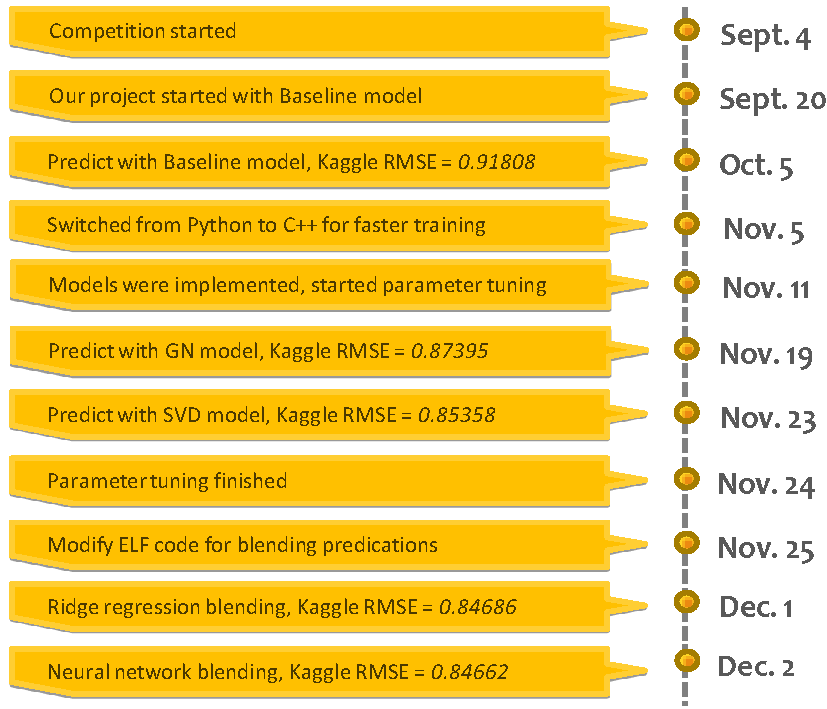
\includegraphics[width=3in]{fig/progress}
\vspace{-2mm}
\caption{Team {\it 1UP+} project progress.}
\label{fig3}
\end{center}
\end{figure}


\begin{table*}[ht]
  \centering
  \begin{tabular}{*{3}{|c}|}
    \hline
    \bf model & \bf mean\_RMSE & \bf description \\ \hline 
    GN & 0.860872 & $\gamma_1 = 0.02, \gamma_3 = 0.05, \lambda_1 = 0.01, \lambda_3 = 0.005$  \\ \hline
    GN & 0.860883 & $\gamma_1 = 0.02, \gamma_3 = 0.05, \lambda_1 = 0.005, \lambda_3 = 0.005$  \\ \hline
    GN & 0.860922 & $\gamma_1 = 0.01, \gamma_3 = 0.05, \lambda_1 = 0.01, \lambda_3 = 0.005$  \\ \hline
    GN & 0.860934 & $\gamma_1 = 0.02, \gamma_3 = 0.05, \lambda_1 = 0.002, \lambda_3 = 0.005$  \\ \hline
    GN & 0.860936 & $\gamma_1 = 0.01, \gamma_3 = 0.05, \lambda_1 = 0.005, \lambda_3 = 0.005$  \\ \hline
    SVD & 0.842237 & $k = 400, \gamma_1 = 0.02, \gamma_2 = 0.04, \lambda_1 = 0.02, \lambda_2 = 0.03$  \\ \hline
    SVD & 0.842259 & $k = 400, \gamma_1 = 0.02, \gamma_2 = 0.04, \lambda_1 = 0.01, \lambda_2 = 0.03$  \\ \hline
    SVD & 0.842287 & $k = 400, \gamma_1 = 0.02, \gamma_2 = 0.04, \lambda_1 = 0.005, \lambda_2 = 0.03$  \\ \hline
    SVD & 0.842289 & $k = 300, \gamma_1 = 0.02, \gamma_2 = 0.04, \lambda_1 = 0.02, \lambda_2 = 0.03$  \\ \hline
    SVD & 0.842310 & $k = 400, \gamma_1 = 0.02, \gamma_2 = 0.04, \lambda_1 = 0.002, \lambda_2 = 0.03$  \\ \hline
    SVDasym & 0.843231 & $k = 300, \gamma_1 = 0.015, \gamma_2 = 0.01, \lambda_1 = 0.005, \lambda_2 = 0.05$  \\ \hline
    SVDasym & 0.843250 & $k = 300, \gamma_1 = 0.01, \gamma_2 = 0.01, \lambda_1 = 0.01, \lambda_2 = 0.05$  \\ \hline
    SVDasym & 0.843265 & $k = 300, \gamma_1 = 0.012, \gamma_2 = 0.015, \lambda_1 = 0.005, \lambda_2 = 0.06$  \\ \hline
    SVDasym & 0.843266 & $k = 300, \gamma_1 = 0.02, \gamma_2 = 0.01, \lambda_1 = 0.001, \lambda_2 = 0.05$  \\ \hline
    SVDasym & 0.843269 & $k = 300, \gamma_1 = 0.01, \gamma_2 = 0.01, \lambda_1 = 0.008, \lambda_2 = 0.05$  \\ \hline
    SVD++ & 0.844711 & $k = 200, \gamma_1 = 0.04, \gamma_2 = 0.022, \lambda_1 = 0.02, \lambda_2 = 0.03$  \\ \hline
    SVD++ & 0.844712 & $k = 200, \gamma_1 = 0.035, \gamma_2 = 0.022, \lambda_1 = 0.02, \lambda_2 = 0.03$  \\ \hline
    SVD++ & 0.844725 & $k = 200, \gamma_1 = 0.03, \gamma_2 = 0.022, \lambda_1 = 0.02, \lambda_2 = 0.03$  \\ \hline
    SVD++ & 0.844745 & $k = 150, \gamma_1 = 0.035, \gamma_2 = 0.022, \lambda_1 = 0.02, \lambda_2 = 0.03$  \\ \hline
    SVD++ & 0.844756 & $k = 150, \gamma_1 = 0.03, \gamma_2 = 0.022, \lambda_1 = 0.02, \lambda_2 = 0.03$  \\ \hline
    SVDGN & 0.840031 & $k = 400, \gamma_1 = 0.05, \gamma_2 = 0.035, \gamma_3 = 0.012, \lambda_1 = 0.01, \lambda_2 = 0.035, \lambda_3 = 0.15$  \\ \hline
    SVDGN & 0.840056 & $k = 400, \gamma_1 = 0.05, \gamma_2 = 0.035, \gamma_3 = 0.012, \lambda_1 = 0.008, \lambda_2 = 0.035, \lambda_3 = 0.15$  \\ \hline
    SVDGN & 0.840101 & $k = 400, \gamma_1 = 0.05, \gamma_2 = 0.035, \gamma_3 = 0.012, \lambda_1 = 0.005, \lambda_2 = 0.035, \lambda_3 = 0.15$  \\ \hline
    SVDGN & 0.840106 & $k = 400, \gamma_1 = 0.04, \gamma_2 = 0.035, \gamma_3 = 0.012, \lambda_1 = 0.01, \lambda_2 = 0.035, \lambda_3 = 0.15$  \\ \hline
    SVDGN & 0.840132 & $k = 400, \gamma_1 = 0.04, \gamma_2 = 0.035, \gamma_3 = 0.012, \lambda_1 = 0.008, \lambda_2 = 0.035, \lambda_3 = 0.15$  \\ \hline
    support & - & The natural logarithm of the number of ratings per user.  \\ \hline
  \end{tabular}
  \vspace{0.15cm}
  \caption{The dataset used for the final predication blending.}
  \label{tab1}
\end{table*}


The Baseline model is evaluated on a wide parameter space of $\gamma_1$ and $\lambda_1$, and the optimal Baseline model is obtained when $\gamma_1 = 0.001$, $\lambda_1 = 0.01$, and number of iteration is $15$, which gives mean\_RMSE 0.906189. This model is not included in the final combination, but the $b_u$ and $b_i$ from this model are used to initialize the $b_u$ and $b_i$ when training other models.

For GN, SVD, SVDasym, SVD++, and SVDGN models, the best 5 parameter sets for each model and the corresponding mean\_RMSE are shown in Table~\ref{tab1}. All models significantly improved the prediction accuracy, compared to Baseline model. The SVD based models (SVD, SVDasym, SVD++) had a better performance than neighborhood based model (GN), and combined neighborhood and SVD model (SVDGN) had smallest mean\_RMSE.

All models listed in Table~\ref{tab1} were included in the final combination, along with the \lq\lq{}support\rq\rq{}, which is the natural logarithm of the number of ratings per user. Blending these 26 inputs with ridge regression could achieve a RMSE of 0.84686 on Kaggle Quiz Set, and blending with neural network reaches a RMSE of 0.84662. The final prediction chosen for Kaggle Test Set is the latter one, and the final result is RMSE = 0.84536.



\section{Conclusion}
The conclusion goes here.


% if have a single appendix:
%\appendix[Proof of the Zonklar Equations]
% or
%\appendix  % for no appendix heading
% do not use \section anymore after \appendix, only \section*
% is possibly needed

% use appendices with more than one appendix
% then use \section to start each appendix
% you must declare a \section before using any
% \subsection or using \label (\appendices by itself
% starts a section numbered zero.)
%


%\appendices
%\section{Proof of the First Zonklar Equation}
%Appendix one text goes here.
%
%% you can choose not to have a title for an appendix
%% if you want by leaving the argument blank
%\section{}
%Appendix two text goes here.


% use section* for acknowledgement
% 

\section*{Acknowledgment}
We would like to thank Dr. Genevera Allen for the wonderful class and competition. We acknowledge the use of the cluster of Computational and Integrative Biomedical Research Center at Baylor College of Medicine and the cluster of Center for Statistical Genetics at Baylor College of Medicine for assistance in computation of this project. We also thank Michael Jahrer for his open software {\it ELF}. 

D.F. and Z.X.H. conceived of the project, implemented the methods and performed parameter tuning. Z.X.H. performed blending and wrote the report.  

% Can use something like this to put references on a page
% by themselves when using endfloat and the captionsoff option.
\ifCLASSOPTIONcaptionsoff
  \newpage
\fi


% trigger a \newpage just before the given reference
% number - used to balance the columns on the last page
% adjust value as needed - may need to be readjusted if
% the document is modified later
%\IEEEtriggeratref{8}
% The "triggered" command can be changed if desired:
%\IEEEtriggercmd{\enlargethispage{-5in}}

% references section

% can use a bibliography generated by BibTeX as a .bbl file
% BibTeX documentation can be easily obtained at:
% http://www.ctan.org/tex-archive/biblio/bibtex/contrib/doc/
% The IEEEtran BibTeX style support page is at:
% http://www.michaelshell.org/tex/ieeetran/bibtex/
%\bibliographystyle{IEEEtran}
% argument is your BibTeX string definitions and bibliography database(s)
%\bibliography{IEEEabrv,../bib/paper}
%
% <OR> manually copy in the resultant .bbl file
% set second argument of \begin to the number of references
% (used to reserve space for the reference number labels box)
\begin{thebibliography}{1}
%\bibitem{tzhou}
%\emph{Recommender Systems}, Physics Reports Vol. 519 (1), P. 1-49 (2012)

\bibitem{koren}
Factorization meets the neighborhood: a multifaceted collaborative filtering model, http://public.research.att.com/~volinsky/netflix/kdd08koren.pdf

\bibitem{item}
Item-Based Collaborative Filtering Recommendation Algorithms, http://www.ra.ethz.ch/cdstore/www10/papers/pdf/p519.pdf

\bibitem{lesson}
Lessons from the Netflix Prize Challenge, http://public.research.att.com/\~volinsky/netflix/sigkddexp.pdf

\bibitem{svd}
Netflix update: Try this at home, http://sifter.org/\~simon/journal/20061211.html

\bibitem{Paterek}
Improving regularized singular value decomposition for collaborative filtering, http://www.cs.uic.edu/~liub/KDD-cup-2007/proceedings/Regular-Paterek.pdf

\bibitem{blend}
Combining Predictions for Accurate Recommender Systems, http://www.commendo.at/UserFiles/commendo/File/kdd2010-paper.pdf


\bibitem{elf}
ELF - ensemble learning framework, http://elf-project.sourceforge.net/

\end{thebibliography}

% biography section
% 
% If you have an EPS/PDF photo (graphicx package needed) extra braces are
% needed around the contents of the optional argument to biography to prevent
% the LaTeX parser from getting confused when it sees the complicated
% \includegraphics command within an optional argument. (You could create
% your own custom macro containing the \includegraphics command to make things
% simpler here.)
%\begin{biography}[{\includegraphics[width=1in,height=1.25in,clip,keepaspectratio]{mshell}}]{Michael Shell}
% or if you just want to reserve a space for a photo:

%\begin{IEEEbiography}{Michael Shell}
%Biography text here.
%\end{IEEEbiography}
%
%% if you will not have a photo at all:
%\begin{IEEEbiographynophoto}{John Doe}
%Biography text here.
%\end{IEEEbiographynophoto}
%
%% insert where needed to balance the two columns on the last page with
%% biographies
%%\newpage
%
%\begin{IEEEbiographynophoto}{Jane Doe}
%Biography text here.
%\end{IEEEbiographynophoto}

% You can push biographies down or up by placing
% a \vfill before or after them. The appropriate
% use of \vfill depends on what kind of text is
% on the last page and whether or not the columns
% are being equalized.

%\vfill

% Can be used to pull up biographies so that the bottom of the last one
% is flush with the other column.
%\enlargethispage{-5in}



% that's all folks
\end{document}


